% Extension 2: CP-Decomposition Slides

\begin{frame}{Extension 2: CP-Decomposition}
    \begin{columns}
        \column{0.5\textwidth}
        \textbf{Motivation:}
        \begin{itemize}
            \item Post-hoc $\to$ \textbf{intrinsic} interpretability
            \item Standard eigendecomposition: orthogonality $\to$ entangled
            \item CP: disentangled features
        \end{itemize}
        
        \vspace{0.2cm}
        \textbf{CP Factorization:}
        \begin{equation*}
            W_{cij} = \sum_{r=1}^{R} \lambda_r A_{cr} B_{ir} C_{jr}
        \end{equation*}
        
        \vspace{0.2cm}
        \textbf{Key Properties:}
        \begin{itemize}
            \item No orthogonality constraint
            \item Disentangled representations
            \item Parameter reduction $\to$ faster training and scalability
        \end{itemize}
        
        \column{0.5\textwidth}
        \begin{figure}
            \centering
            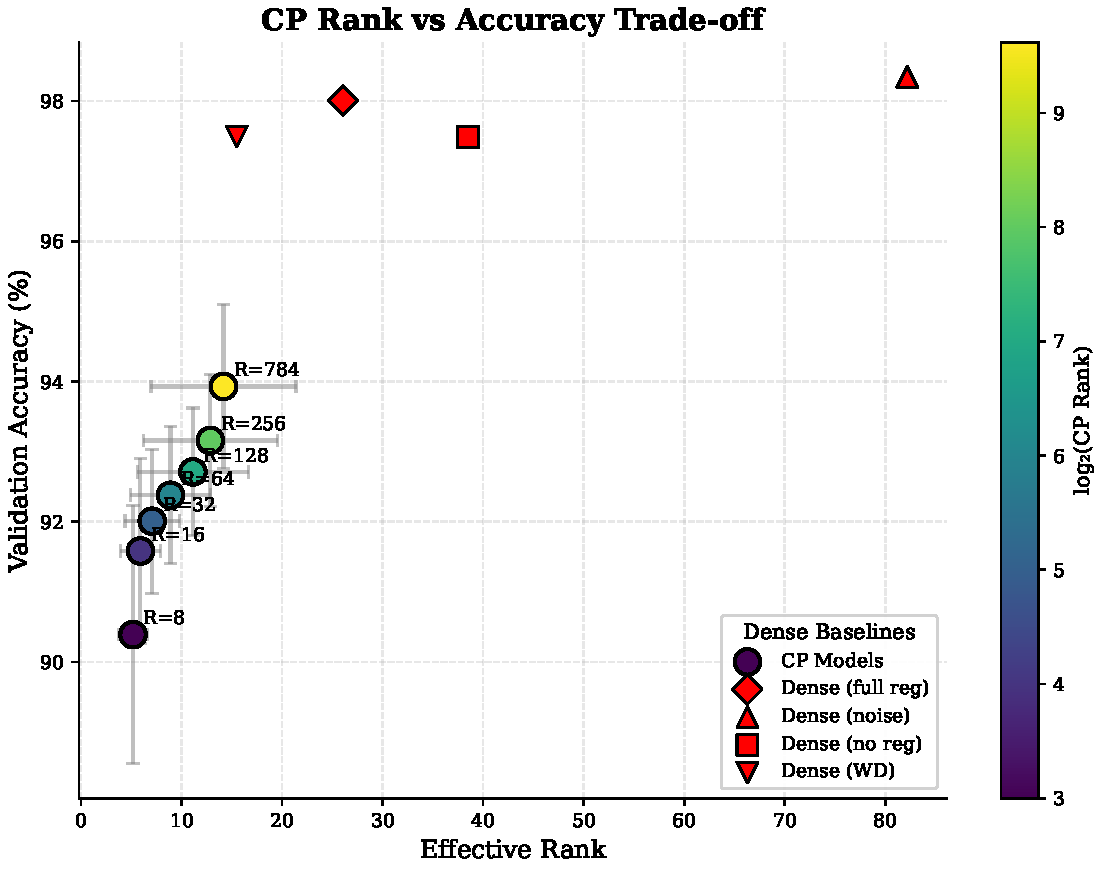
\includegraphics[width=0.95\textwidth]{../Report/figures/extension_cp/cp_rank_accuracy_tradeoff.pdf}
            \caption{Accuracy vs rank trade-off}
        \end{figure}
        
        \vspace{0.2cm}
        \textbf{Results at $R=256$:}
        \begin{itemize}
            \item Accuracy: \textbf{93.8\%}
            \item Effective rank: \textbf{17.5}
            \item vs Dense: 97.5\% (3.7 pp drop)
        \end{itemize}
    \end{columns}
\end{frame}

\begin{frame}{CP-Decomposition: Efficiency}
    \begin{center}
        \begin{table}
            \centering
            \small
            \begin{tabular}{lcccc}
                \toprule
                Experiment & Runs & Wall (h) & GPU-h & CO2 (kg) \\
                \midrule
                Vision (Section 4)$^\dagger$ & 81 & 1.22 & 1.11 & 0.039 \\
                Language (Section 5)$^\ddagger$ & 3 & 19.09 & 0.00 & 0.105 \\
                Extension 1 & 15 & 0.58 & 0.58 & 0.020 \\
                Extension 2 (CP) & 105 & 0.05 & 0.05 & 0.004 \\
                \midrule
                \textbf{Total} & \textbf{204} & \textbf{20.95} & \textbf{1.74} & \textbf{0.168} \\
                \bottomrule
            \end{tabular}
            \caption{Environmental impact (CO2 via \texttt{codecarbon})}
        \end{table}
        
        
        
    \end{center}
    
    \vspace{0.3cm}
    \textbf{Key Efficiency Gains:}
    \begin{itemize}
        \item \textbf{Parameter reduction:} $\mathcal{O}(d_{\text{hidden}} \times d_{\text{in}}^2) \to \mathcal{O}(R \times d_{\text{in}})$
        \item Average GPU-h per run: CP decomposition (0.00048) vs Vision (0.014) --- \textbf{29$\times$ more efficient}
        \item Only \textbf{3.7 pp accuracy drop} for significant parameter efficiency
    \end{itemize}
\end{frame}

\begin{frame}{CP-Decomposition: Disentangled Factors}
    \begin{figure}
        \centering
        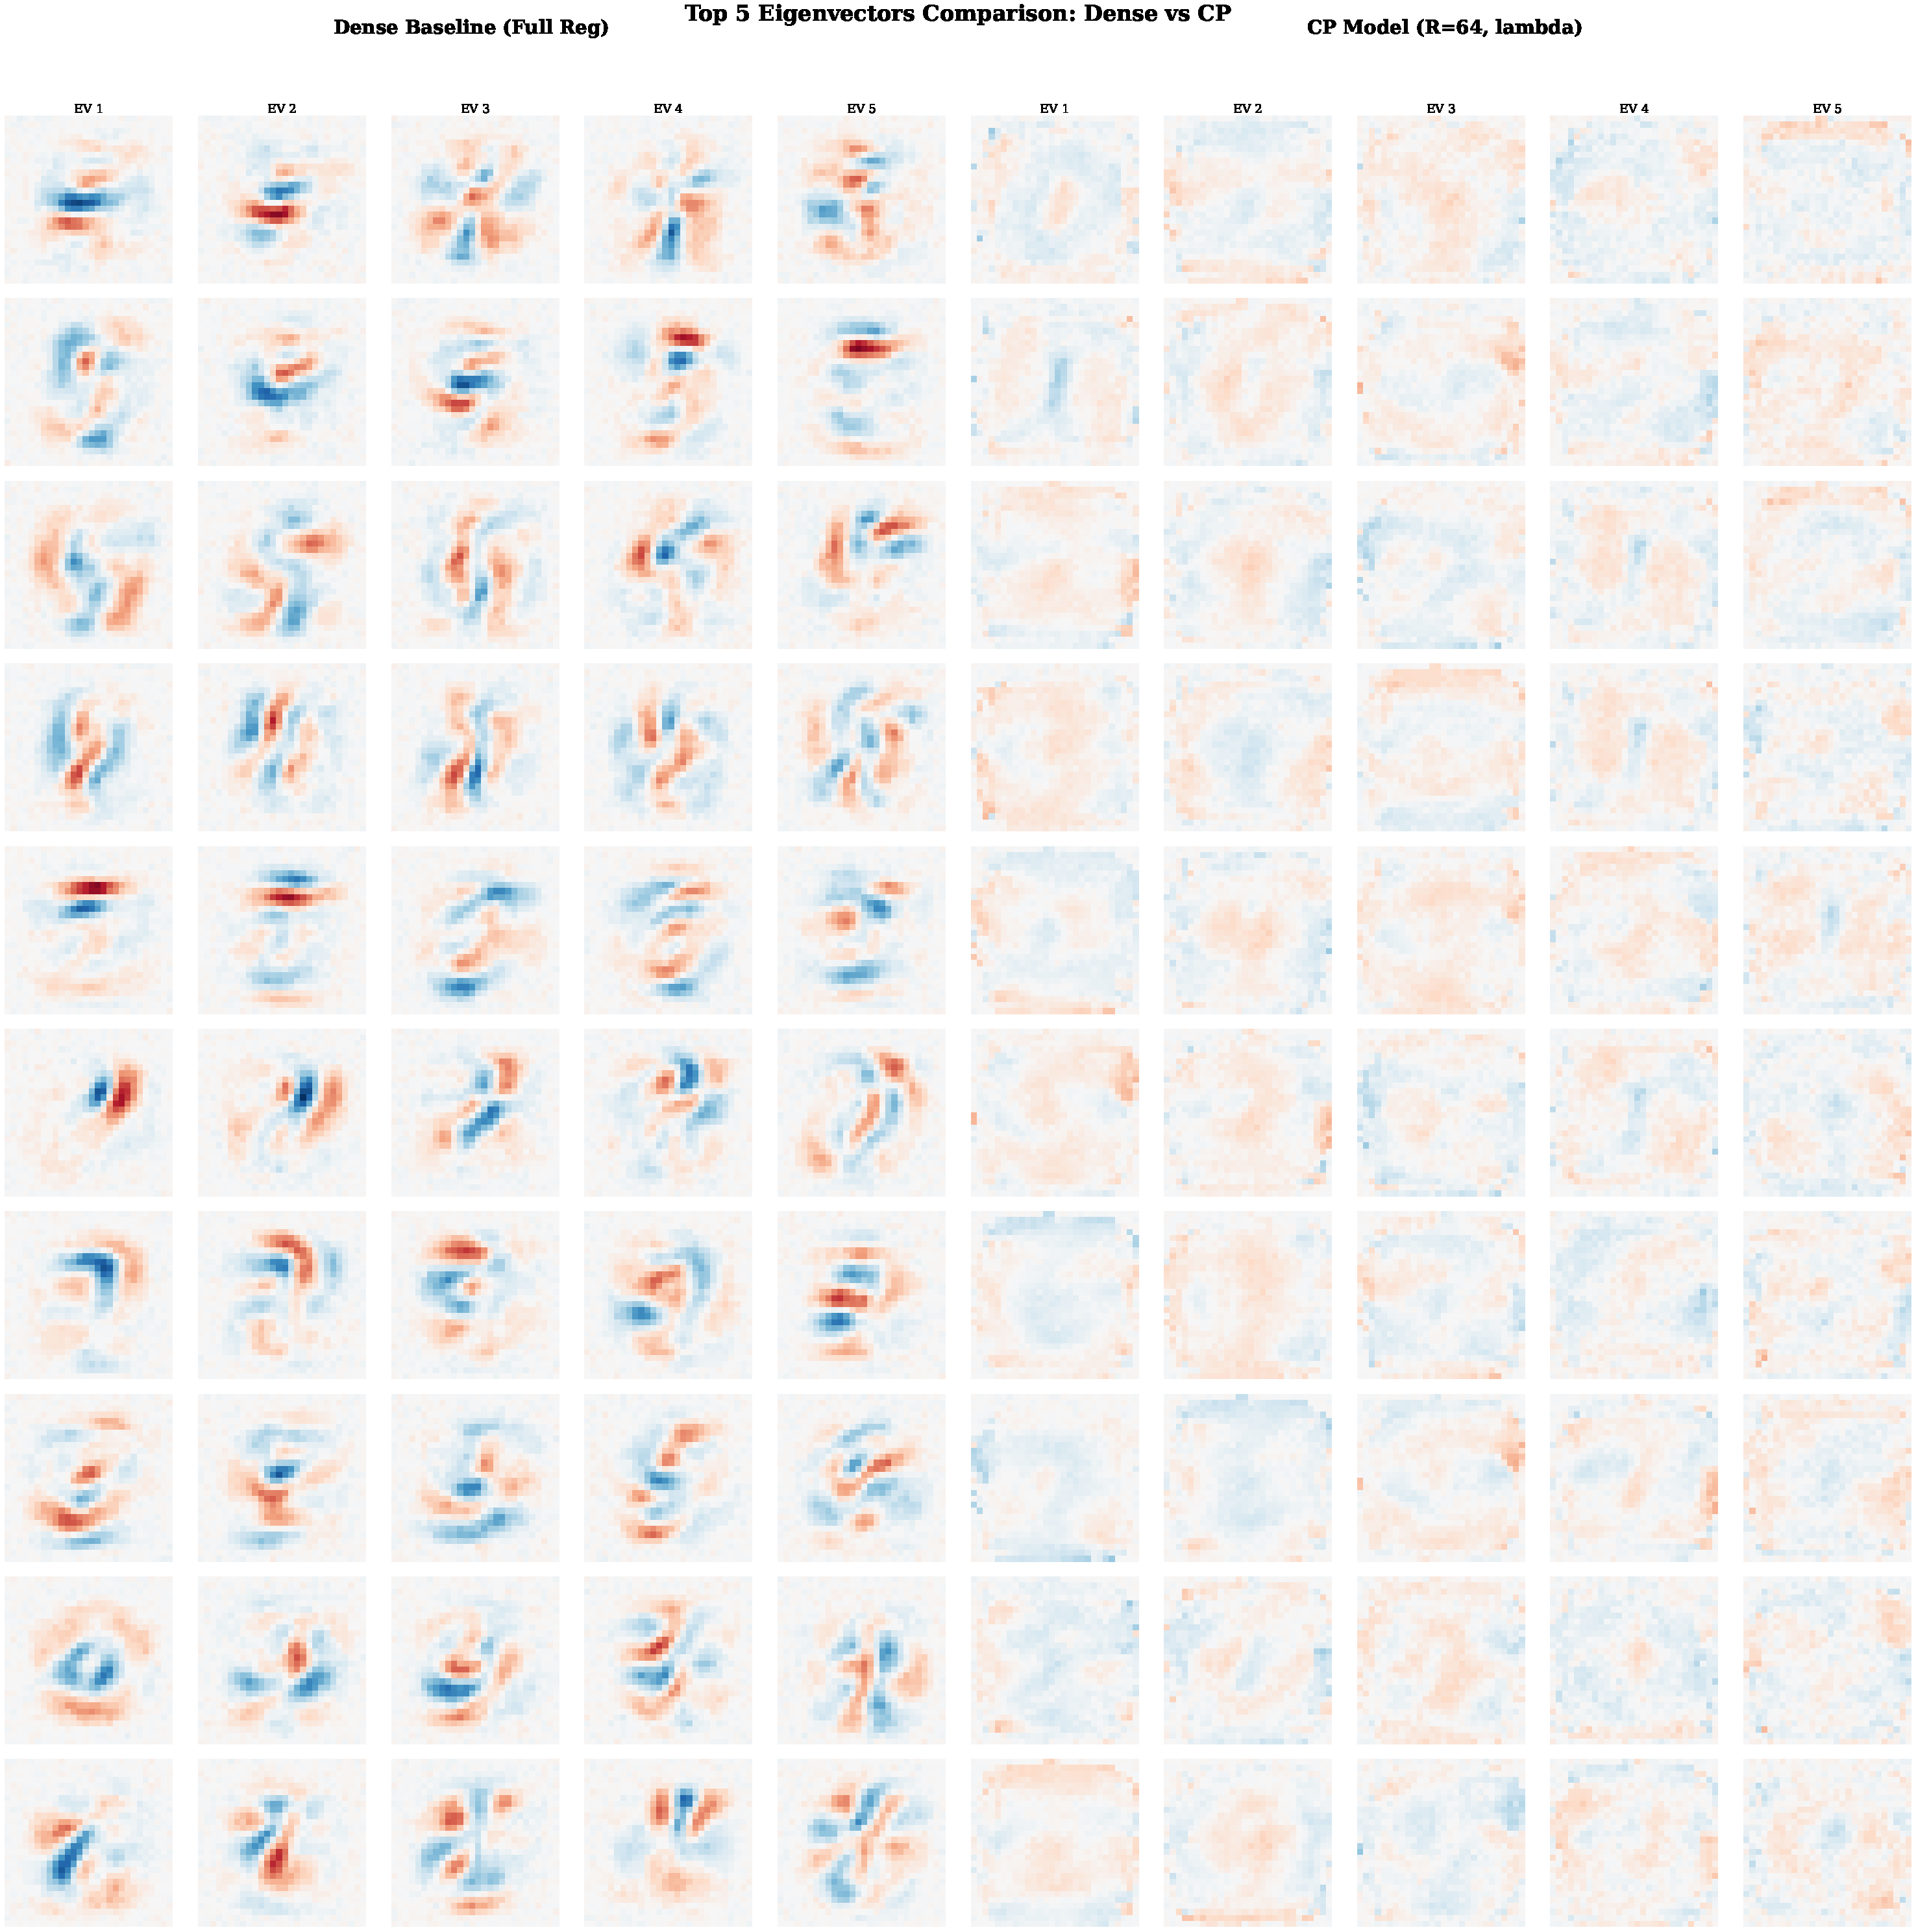
\includegraphics[width=0.65\textwidth,height=0.45\textheight,keepaspectratio]{../Report/figures/extension_cp/cp_top5_eigenvectors_comparison.pdf}
        \caption{Feature disentanglement: Dense vs.\ CP}
    \end{figure}
    
    \vspace{-0.2cm}
    \begin{columns}
        \column{0.5\textwidth}
        \small
        \textbf{Dense Eigenvectors:}
        \begin{itemize}
            \item Holistic, superimposed templates
            \item Entangled representations
        \end{itemize}
        
        \column{0.5\textwidth}
        \small
        \textbf{CP Factors:}
        \begin{itemize}
            \item Atomic, localized factors
            \item ``Parts-based'' representations
        \end{itemize}
    \end{columns}
\end{frame}

\begin{frame}
    \centering
    \vspace{2cm}
    {\Huge \textbf{Thank You!}}
    
    \vspace{1.5cm}
    {\large Questions?}
    
    \vspace{1.5cm}
    \small
    Itay Erlich, May Ben Zion, Jacob Shashoua, Sagi Schwartz
    
    \vspace{0.3cm}
    \footnotesize
    FACT-AI Course Project, University of Amsterdam
\end{frame}
